\documentclass[]{scrartcl}
\usepackage[T1]{fontenc}
\usepackage{lmodern}
\usepackage{amssymb,amsmath}
\usepackage{ifxetex,ifluatex}
\usepackage[svgnames]{xcolor} % Enabling colors by their 'svgnames'
\usepackage{fixltx2e} % provides \textsubscript
% use microtype if available
\IfFileExists{microtype.sty}{\usepackage{microtype}}{}
% use upquote if available, for straight quotes in verbatim environments
\IfFileExists{upquote.sty}{\usepackage{upquote}}{}
\ifnum 0\ifxetex 1\fi\ifluatex 1\fi=0 % if pdftex
  \usepackage[utf8]{inputenc}
\else % if luatex or xelatex
  \usepackage{fontspec}
  \ifxetex
    \usepackage{xltxtra,xunicode}
  \fi
  \defaultfontfeatures{Mapping=tex-text,Scale=MatchLowercase}
  \newcommand{\euro}{€}
\fi
\usepackage{color}
\usepackage{fancyvrb}
\newcommand{\VerbBar}{|}
\newcommand{\VERB}{\Verb[commandchars=\\\{\}]}
\DefineVerbatimEnvironment{Highlighting}{Verbatim}{commandchars=\\\{\}}
% Add ',fontsize=\small' for more characters per line
\newenvironment{Shaded}{}{}
\newcommand{\KeywordTok}[1]{\textcolor[rgb]{0.00,0.44,0.13}{\textbf{{#1}}}}
\newcommand{\DataTypeTok}[1]{\textcolor[rgb]{0.56,0.13,0.00}{{#1}}}
\newcommand{\DecValTok}[1]{\textcolor[rgb]{0.25,0.63,0.44}{{#1}}}
\newcommand{\BaseNTok}[1]{\textcolor[rgb]{0.25,0.63,0.44}{{#1}}}
\newcommand{\FloatTok}[1]{\textcolor[rgb]{0.25,0.63,0.44}{{#1}}}
\newcommand{\CharTok}[1]{\textcolor[rgb]{0.25,0.44,0.63}{{#1}}}
\newcommand{\StringTok}[1]{\textcolor[rgb]{0.25,0.44,0.63}{{#1}}}
\newcommand{\CommentTok}[1]{\textcolor[rgb]{0.38,0.63,0.69}{\textit{{#1}}}}
\newcommand{\OtherTok}[1]{\textcolor[rgb]{0.00,0.44,0.13}{{#1}}}
\newcommand{\AlertTok}[1]{\textcolor[rgb]{1.00,0.00,0.00}{\textbf{{#1}}}}
\newcommand{\FunctionTok}[1]{\textcolor[rgb]{0.02,0.16,0.49}{{#1}}}
\newcommand{\RegionMarkerTok}[1]{{#1}}
\newcommand{\ErrorTok}[1]{\textcolor[rgb]{1.00,0.00,0.00}{\textbf{{#1}}}}
\newcommand{\NormalTok}[1]{{#1}}
\usepackage{longtable}
\let\oldlongtable\longtable

\def\longtable{\tiny \oldlongtable}


\usepackage{libertine}
\usepackage{framed}
\let\oldquote\quote
\let\endoldquote\endquote
\definecolor{verypalegreen}{RGB}{252,255,250}
\colorlet{shadecolor}{verypalegreen}

\makeatletter
\def\shadequote{\begin{snugshade}\begin{oldquote}}
\def\endshadequote{%
  \end{oldquote}\end{snugshade}}
\makeatother
  
\renewenvironment{quote}{\begin{shadequote}}{\end{shadequote}}
\usepackage{graphicx}
% We will generate all images so they have a width \maxwidth. This means
% that they will get their normal width if they fit onto the page, but
% are scaled down if they would overflow the margins.
\makeatletter
\def\maxwidth{\ifdim\Gin@nat@width>\linewidth\linewidth
\else\Gin@nat@width\fi}
\makeatother
\let\Oldincludegraphics\includegraphics
\renewcommand{\includegraphics}[1]{\Oldincludegraphics[width=\maxwidth]{#1}}
\ifxetex
  \usepackage[setpagesize=false, % page size defined by xetex
              unicode=false, % unicode breaks when used with xetex
              xetex]{hyperref}
\else
  \usepackage[unicode=true]{hyperref}
\fi
\hypersetup{breaklinks=true,
            bookmarks=true,
            pdfauthor={James Hetherington},
            pdftitle={Practical Version Control and Issue Tracking},
            colorlinks=true,
            urlcolor=blue,
            linkcolor=uclmidgreen,
            pdfborder={0 0 0}}
\urlstyle{same}  % don't use monospace font for urls
% Make links footnotes instead of hotlinks:
\renewcommand{\href}[2]{#2\footnote{\url{#1}}}
\setlength{\parindent}{0pt}
\setlength{\parskip}{6pt plus 2pt minus 1pt}
\setlength{\emergencystretch}{3em}  % prevent overfull lines
  
\usepackage{lettrine} % Package to accentuate the first letter of the text  
\usepackage{fix-cm}	 % Custom font sizes - used for the initial letter in the document

\definecolor{uclmidgreen}{RGB}{130,141,55}

\newcommand{\initial}[1]{ % Defines the command and style for the first letter
\lettrine[lines=3,lhang=0.3,nindent=0em]{
\color{DarkGreen}
{\textsf{#1}}}{}}

\usepackage{sectsty} % Enables custom section titles
\sectionfont{\color{uclmidgreen} \usefont{OT1}{phv}{b}{n}} % Change the font of all section commands
\subsectionfont{\color{DarkSeaGreen} \usefont{OT1}{phv}{b}{n}} % Change the font of all section commands

\usepackage{titling} % Allows custom title configuration 
\newcommand{\HorRule}{\color{DarkSeaGreen} \rule{\linewidth}{1pt}} % Defines the gold horizontal rule around the title

\pretitle{
\vspace{-30pt} \begin{flushleft} \HorRule \fontsize{38}{38} \usefont{OT1}{phv}{b}{n} \color{uclmidgreen} \selectfont} % Horizontal rule before the title

\posttitle{\par\end{flushleft}\begin{flushleft}\fontsize{35}{35} \usefont{OT1}{phv}{b}{n} \color{Black} \selectfont  \end{flushleft}\vskip 0.5em} % Whitespace under the title and subtitle

\preauthor{\begin{flushleft}\large \lineskip 0.5em \usefont{OT1}{phv}{b}{sl} \color{uclmidgreen}} % Author font configuration
\title{Practical Version Control and Issue Tracking}


\author{James Hetherington}
\date{}

\postauthor{\footnotesize \usefont{OT1}{phv}{m}{sl} \color{Black} % Configuration for the institution name


University College London% Your institution

\par\end{flushleft}\HorRule} % Horizontal rule after the title
      

\usepackage{picture}
\usepackage{eso-pic}

\begin{document}
  \AddToShipoutPicture{\put(0,\dimexpr\paperheight-1.8cm){%
    \makebox[\paperwidth]{\Oldincludegraphics[width=\paperwidth,height=1.8cm]{assets/bannermidgreen.pdf}}%
  }}

\maketitle

\section{Practical Version Control and Issue
Tracking}\label{practical-version-control-and-issue-tracking}

\subsection{What Version Control is
For}\label{what-version-control-is-for}

\begin{itemize}
\itemsep1pt\parskip0pt\parsep0pt
\item
  Managing Code Inventory

  \begin{itemize}
  \itemsep1pt\parskip0pt\parsep0pt
  \item
    ``When did I introduce this bug''?
  \item
    Undoing Mistakes
  \end{itemize}
\item
  Working with other programmers

  \begin{itemize}
  \itemsep1pt\parskip0pt\parsep0pt
  \item
    ``How can I merge my work with Jim's''
  \end{itemize}
\end{itemize}

\subsection{What is version control?}\label{what-is-version-control}

Do some programming

\texttt{my\_vcs commit}

Program some more

Realise mistake

\texttt{my\_vcs rollback}

Mistake is undone

\subsection{What is version control? (Team
version)}\label{what-is-version-control-team-version}

\begin{longtable}[c]{@{}lr@{}}
\hline\noalign{\medskip}
Sue & James
\\\noalign{\medskip}
\hline\noalign{\medskip}
Create some code &
\\\noalign{\medskip}
\texttt{my\_vcs commit} &
\\\noalign{\medskip}
& Join the team
\\\noalign{\medskip}
& \texttt{my\_vcs checkout}
\\\noalign{\medskip}
& do some programming
\\\noalign{\medskip}
& \texttt{my\_vcs commit}
\\\noalign{\medskip}
\texttt{my\_vcs update} & more programming
\\\noalign{\medskip}
Do some programming &
\\\noalign{\medskip}
& \texttt{my\_vcs commit}
\\\noalign{\medskip}
\texttt{my\_vcs commit} &
\\\noalign{\medskip}
Oh Noes! Error! &
\\\noalign{\medskip}
\texttt{my\_vcs update} &
\\\noalign{\medskip}
\texttt{my\_vcs merge} &
\\\noalign{\medskip}
\texttt{my\_vcs commit} &
\\\noalign{\medskip}
& \texttt{my\_vcs commit}
\\\noalign{\medskip}
& Error again\ldots{}
\\\noalign{\medskip}
\hline
\end{longtable}

\section{Centralised Version Control}\label{centralised-version-control}

\subsection{Centralised VCS concepts}\label{centralised-vcs-concepts}

\begin{itemize}
\itemsep1pt\parskip0pt\parsep0pt
\item
  There is one, linear history of changes on the server or
  \textbf{repository}
\item
  Each revision has a unique, sequential identifier (1,2,3,4\ldots{})
\item
  You have a \textbf{working copy}
\item
  You \textbf{update} the working copy to match the state of the
  repository
\item
  If someone else has changed the repository while you were working:
\item
  You update to get their changes
\item
  You have to \textbf{resolve conflicts}
\item
  Then you commit
\end{itemize}

\subsection{Centralised VCS diagram}\label{centralised-vcs-diagram}

\begin{figure}[htbp]
\centering
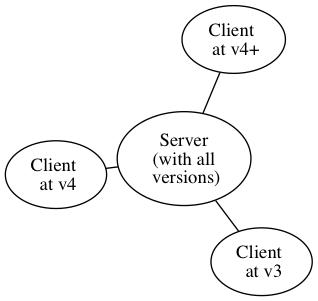
\includegraphics{assets/centralised.png}
\caption{A centralised server with three clients}
\end{figure}

\subsection{Centralised VCS solo
workflow}\label{centralised-vcs-solo-workflow}

\begin{figure}[htbp]
\centering
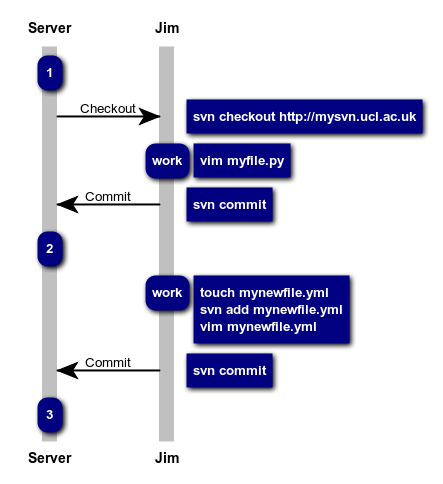
\includegraphics{assets/centralised_solo.png}
\caption{Solo workflow for SVN}
\end{figure}

\subsection{Centralised VCS team
workflow}\label{centralised-vcs-team-workflow}

\begin{figure}[htbp]
\centering
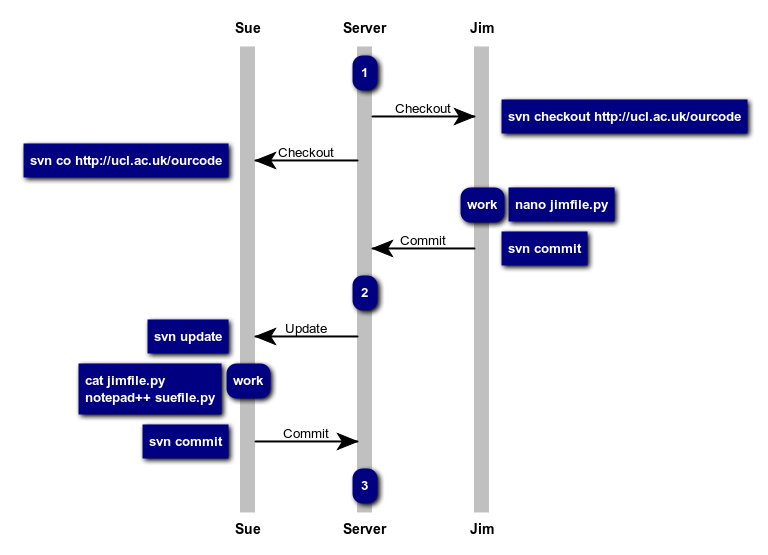
\includegraphics{assets/centralised_team_noconflict.png}
\caption{Team workflow for SVN}
\end{figure}

\subsection{Centralised VCS conflicted
workflow}\label{centralised-vcs-conflicted-workflow}

\begin{figure}[htbp]
\centering
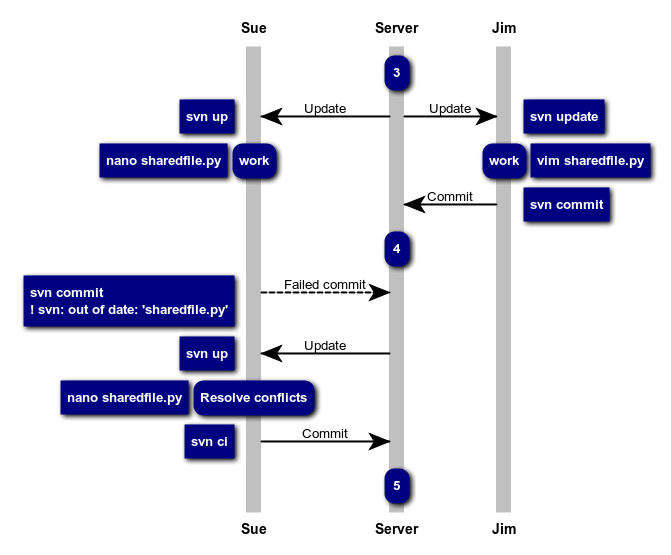
\includegraphics{assets/centralised_team.png}
\caption{Conflicted workflow for SVN}
\end{figure}

\subsection{Resolving conflicts}\label{resolving-conflicts}

On update, you get a prompt like:

\begin{Shaded}
\begin{Highlighting}[]
\KeywordTok{svn} \NormalTok{update}
\KeywordTok{>} \KeywordTok{Conflict} \NormalTok{discovered in ’sharedfile.py}\StringTok{'. }
\StringTok{> Select: (p) postpone, (e) edit, (mc) mine-conflict ...}
\end{Highlighting}
\end{Shaded}

If you choose \texttt{(e)} the conflicted file will look something like:

\begin{Shaded}
\begin{Highlighting}[]
\NormalTok{Whatever was in the file before the conflicted bit}
\StringTok{<<<<<<< .mine}
\NormalTok{Sue’s content}
\KeywordTok{======= }
\NormalTok{Jim’s content}
\OtherTok{>>>>>>> .r4}
\NormalTok{Content after the conflicted bit}
\end{Highlighting}
\end{Shaded}

It is your duty to edit this to fix conflicts, then save.

\subsection{Revisiting history}\label{revisiting-history}

Update to a particular revision:

\begin{Shaded}
\begin{Highlighting}[]
\KeywordTok{svn} \NormalTok{up -r 3}
\end{Highlighting}
\end{Shaded}

See the differences between your working area and a revision

\begin{Shaded}
\begin{Highlighting}[]
\KeywordTok{svn} \NormalTok{diff }\CommentTok{#To most recent version}
\KeywordTok{svn} \NormalTok{diff -r 3}
\end{Highlighting}
\end{Shaded}

See what you've changed:

\begin{Shaded}
\begin{Highlighting}[]
\KeywordTok{svn} \NormalTok{status}
\end{Highlighting}
\end{Shaded}

Get rid of changes to a file:

\begin{verbatim}
svn revert myfile.py
\end{verbatim}

\section{Distributed Version Control}\label{distributed-version-control}

\subsection{Distributed versus
centralised}\label{distributed-versus-centralised}

\begin{longtable}[c]{@{}ll@{}}
\hline\noalign{\medskip}
Centralised & Distributed
\\\noalign{\medskip}
\hline\noalign{\medskip}
Server has history & Every user has full history
\\\noalign{\medskip}
Your computer has one snapshot & Many local branches
\\\noalign{\medskip}
To access history, need internet & History always available
\\\noalign{\medskip}
You commit to remote server & Users synchronise histories
\\\noalign{\medskip}
cvs, subversion(svn) & git, mercurial (hg), bazaar (bzr)
\\\noalign{\medskip}
\hline
\end{longtable}

\subsection{Distributed VCS in
principle}\label{distributed-vcs-in-principle}

\begin{figure}[htbp]
\centering
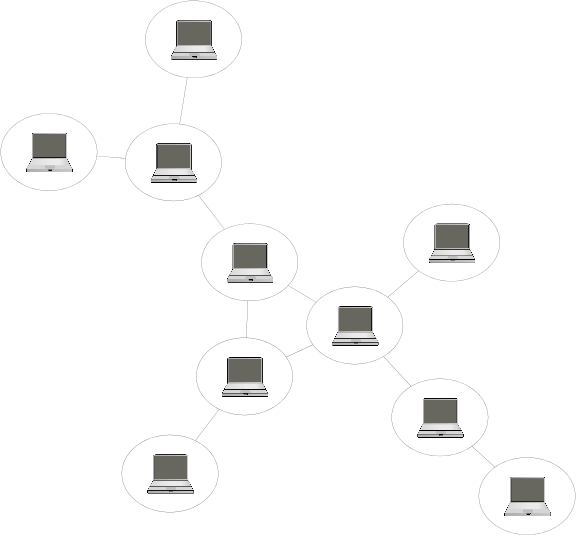
\includegraphics{assets/distributed_principle.png}
\caption{How distributed VCS works in principle}
\end{figure}

\subsection{Distributed VCS in
practice}\label{distributed-vcs-in-practice}

\begin{figure}[htbp]
\centering
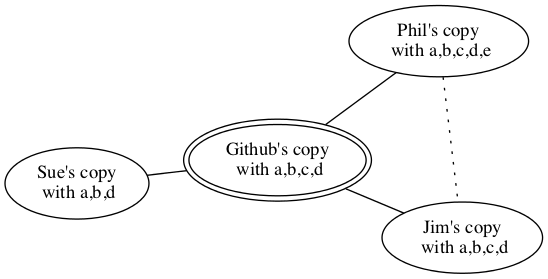
\includegraphics{assets/distributed_practice.png}
\caption{How distributed VCS works in practice}
\end{figure}

\subsection{Pragmatic Distributed VCS}\label{pragmatic-distributed-vcs}

\begin{longtable}[c]{@{}ll@{}}
\hline\noalign{\medskip}
Subversion & Git
\\\noalign{\medskip}
\hline\noalign{\medskip}
\texttt{svn checkout \textless{}URL\textgreater{}} &
\texttt{git clone \textless{}URL\textgreater{}}
\\\noalign{\medskip}
\texttt{svn commit} & \texttt{git commit -a; git push}
\\\noalign{\medskip}
\texttt{svn up} & \texttt{git pull}
\\\noalign{\medskip}
\texttt{svn status} & \texttt{git status}
\\\noalign{\medskip}
\texttt{svn diff} & \texttt{git diff}
\\\noalign{\medskip}
\hline
\end{longtable}

\subsection{Why Go Distributed?}\label{why-go-distributed}

\begin{itemize}
\itemsep1pt\parskip0pt\parsep0pt
\item
  Easy to start a repository (no server needed)
\item
  Easy to start a server
\item
  Can work without internets
\item
  Better merges
\item
  Easy branching
\item
  More widespread support
\end{itemize}

\subsection{Why Not Go Distributed?}\label{why-not-go-distributed}

\begin{itemize}
\itemsep1pt\parskip0pt\parsep0pt
\item
  More complex commands
\item
  More confusing
\end{itemize}

\subsection{Distributed VCS concepts}\label{distributed-vcs-concepts}

\begin{itemize}
\itemsep1pt\parskip0pt\parsep0pt
\item
  Each revision has a parent that it is based on
\item
  These revisions form a graph
\item
  The most recent revision in each copy is the HEAD
\item
  Each revision has a unique hash code
\item
  In Sue's copy, revision 43 is ab3578d6
\item
  Jim thinks that is revision 38
\item
  When you \emph{pull} from a \emph{remote} the histories might conflict
\item
  Histories are \emph{merged} together
\end{itemize}

\subsection{A revision graph}\label{a-revision-graph}

\begin{figure}[htbp]
\centering
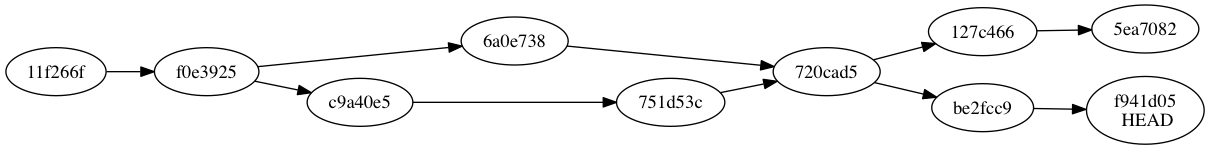
\includegraphics{assets/revisions.png}
\caption{Revisions form a graph}
\end{figure}

\subsection{Distributed VCS concepts
(2)}\label{distributed-vcs-concepts-2}

\begin{itemize}
\itemsep1pt\parskip0pt\parsep0pt
\item
  You have a \emph{working copy}
\item
  You pick a subset of the changes in your working copy to add to the
  next commit
\item
  Changes to be included in the next commit are kept in a
  \textbf{staging area} (a.k.a. \textbf{index})
\item
  When you commit you commit:
\item
  From the staging area
\item
  To the local repository
\item
  You \textbf{push} to \textbf{remote} repositories to share or publish
\item
  You \textbf{pull} (or fetch) to bring in changes from a remote
\end{itemize}

\subsection{The Levels of Git}\label{the-levels-of-git}

\begin{figure}[htbp]
\centering
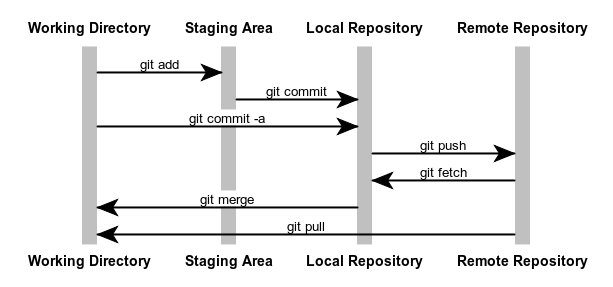
\includegraphics{assets/distributed_concepts.png}
\caption{The relationship between the staging area, working directory,
and repositories in git.}
\end{figure}

\section{Using Git}\label{using-git}

\subsection{Distributed VCS Solo
Workflow}\label{distributed-vcs-solo-workflow}

\begin{figure}[htbp]
\centering
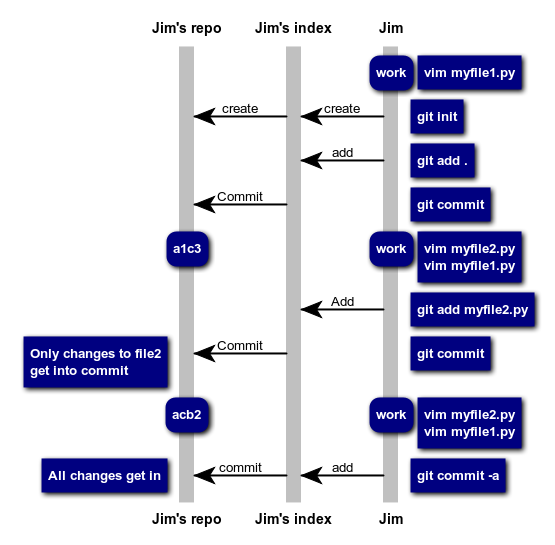
\includegraphics{assets/distributed_solo.png}
\caption{Working alone with git}
\end{figure}

\subsection{Distributed VCS With
Publishing}\label{distributed-vcs-with-publishing}

\begin{figure}[htbp]
\centering
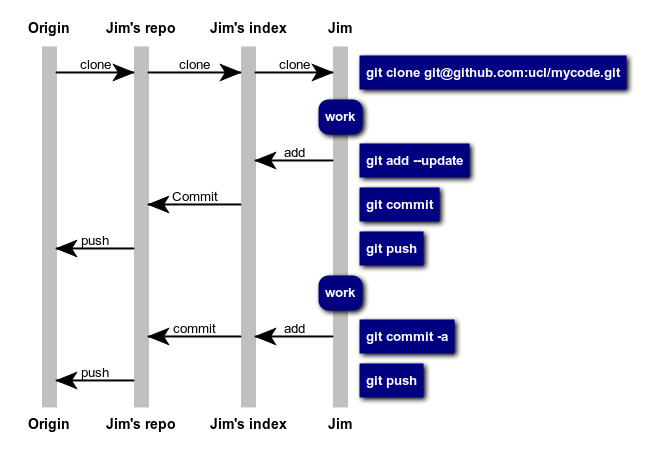
\includegraphics{assets/distributed_solo_publishing.png}
\caption{Publishing with git}
\end{figure}

\subsection{Distributed VCS in teams without
conflicts}\label{distributed-vcs-in-teams-without-conflicts}

\begin{figure}[htbp]
\centering
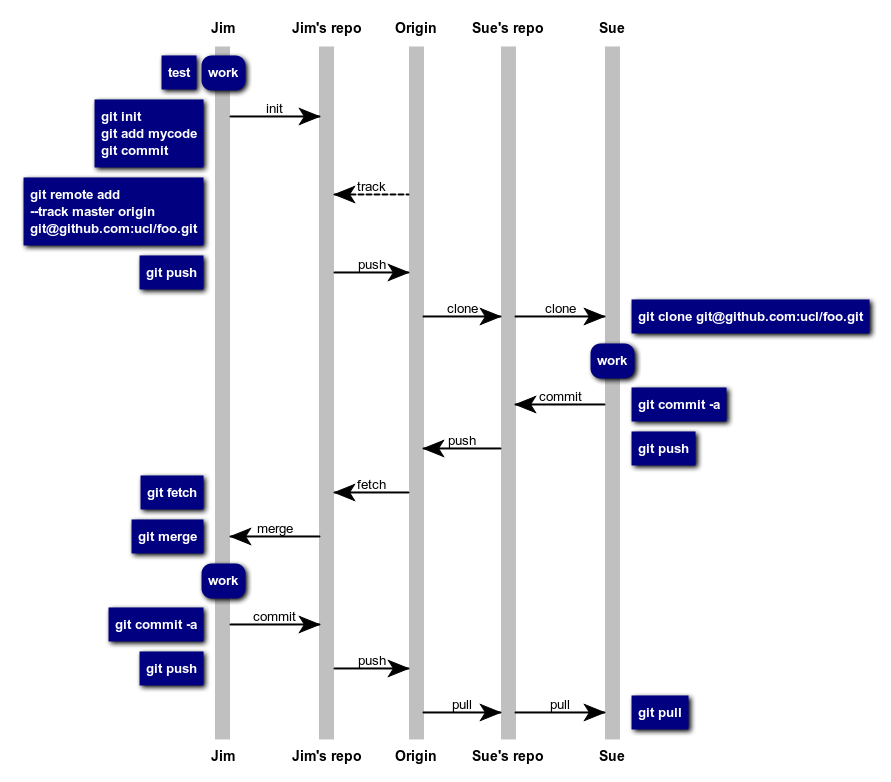
\includegraphics{assets/distributed_shared_noconflict.png}
\caption{Teamworking in git}
\end{figure}

\subsection{Distributed VCS in teams with
conflicts}\label{distributed-vcs-in-teams-with-conflicts}

\begin{figure}[htbp]
\centering
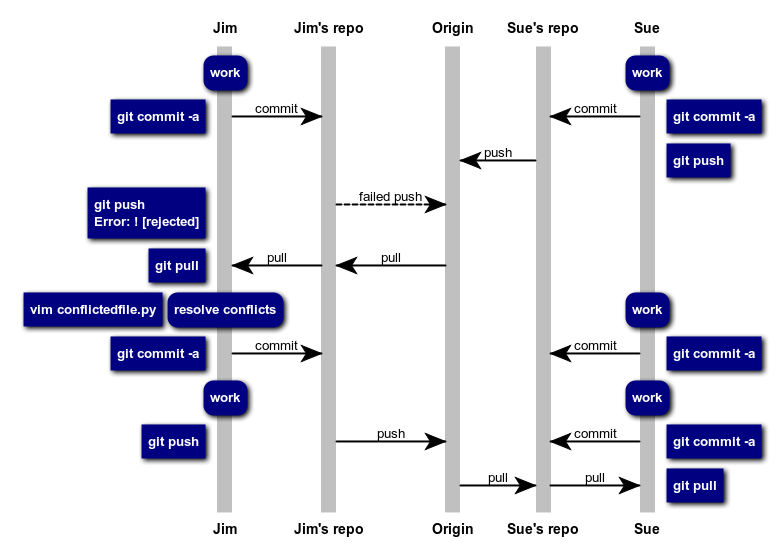
\includegraphics{assets/distributed_shared_conflicted.png}
\caption{Teamworking in git with conflicts}
\end{figure}

\subsection{Working with multiple
remotes}\label{working-with-multiple-remotes}

\begin{Shaded}
\begin{Highlighting}[]
\KeywordTok{git} \NormalTok{remote add sue ssh://sue.ucl.ac.uk/somerepo}
   \CommentTok{# Add a second remote}
\KeywordTok{git} \NormalTok{remote}
   \CommentTok{# List available remotes}
\KeywordTok{git} \NormalTok{push sue}
   \CommentTok{# Push to a specific remote}
   \CommentTok{# Default is origin}
\end{Highlighting}
\end{Shaded}

\section{Branches}\label{branches}

\subsection{Working with branches}\label{working-with-branches}

\begin{figure}[htbp]
\centering
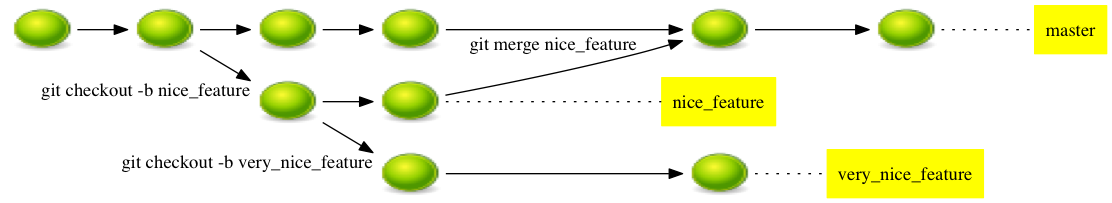
\includegraphics{assets/branching.png}
\caption{Using branches}
\end{figure}

\subsection{Working with branches in
git}\label{working-with-branches-in-git}

\begin{Shaded}
\begin{Highlighting}[]
\KeywordTok{git} \NormalTok{branch }\CommentTok{# Tell me what branches exist}
\end{Highlighting}
\end{Shaded}

\begin{verbatim}
   * master # Asterisk tells me which one
     experiment # I am currently on
\end{verbatim}

\begin{Shaded}
\begin{Highlighting}[]
\KeywordTok{git} \NormalTok{checkout -b somebranch }\CommentTok{# Make a new branch}
\KeywordTok{git} \NormalTok{checkout master }\CommentTok{# Switch to an existing branch}
\end{Highlighting}
\end{Shaded}

\subsection{Sharing branches}\label{sharing-branches}

\begin{Shaded}
\begin{Highlighting}[]
\KeywordTok{git} \NormalTok{push -u origin experiment }\CommentTok{# Share a recently}
                              \CommentTok{# made branch}
\KeywordTok{git} \NormalTok{push origin experiment }\CommentTok{#Republish a branch}
\KeywordTok{git} \NormalTok{branch -r }\CommentTok{#Discover remote branches}
\KeywordTok{git} \NormalTok{checkout origin/some_branch }\CommentTok{#Get a branch}
                                \CommentTok{#from a remote}
\end{Highlighting}
\end{Shaded}

\subsection{Merging branches}\label{merging-branches}

\begin{Shaded}
\begin{Highlighting}[]
\KeywordTok{git} \NormalTok{checkout master }\CommentTok{# Switch to master branch}
\KeywordTok{git} \NormalTok{merge experiment }\CommentTok{# Merge the branch in}
\KeywordTok{git} \NormalTok{branch -d experiment }\CommentTok{# Delete branch locally}
\KeywordTok{git} \NormalTok{push --delete experiment }\CommentTok{# Delete published branch}
\end{Highlighting}
\end{Shaded}

\subsection{A good branch strategy}\label{a-good-branch-strategy}

\begin{itemize}
\itemsep1pt\parskip0pt\parsep0pt
\item
  A \texttt{production} branch: code used for active work
\item
  A \texttt{develop} branch: for general new code
\item
  \texttt{feature} branches: for specific new ideas
\item
  \texttt{release} branches: when you share code with others
\item
  Useful for isolated bug fixes
\end{itemize}

\subsection{Tagging}\label{tagging}

Easy to read labels for revisions Produce real results \emph{only} with
tagged revisions

\begin{Shaded}
\begin{Highlighting}[]
\KeywordTok{git} \NormalTok{tag -a v1.3}
\KeywordTok{git} \NormalTok{push --tags}
\end{Highlighting}
\end{Shaded}

\subsection{Branching and tagging in
subversion}\label{branching-and-tagging-in-subversion}

\begin{itemize}
\itemsep1pt\parskip0pt\parsep0pt
\item
  Subversion doesn't have real branches and tags
\item
  Instead, each is a separate whole copy
\item
  But you can still merge between copies
\end{itemize}

\section{Hosting Servers}\label{hosting-servers}

\subsection{Hosting a server}\label{hosting-a-server}

\begin{itemize}
\itemsep1pt\parskip0pt\parsep0pt
\item
  Any repository can be a remote for pulls
\item
  Can pull/push over shared folders or ssh
\item
  Pushing to someone's working copy is dangerous
\item
  Use \texttt{git init -{}-bare} to make a copy for pushing
\item
  You don't need to create a ``server''
\end{itemize}

\subsection{Hosting a server in the
cloud}\label{hosting-a-server-in-the-cloud}

\begin{itemize}
\itemsep1pt\parskip0pt\parsep0pt
\item
  Many online services
\item
  Github, bitbucket, sourceforge\ldots{}
\item
  I recommend GitHub
\end{itemize}

\end{document}
